\begin{figure}[H]
    \centering
    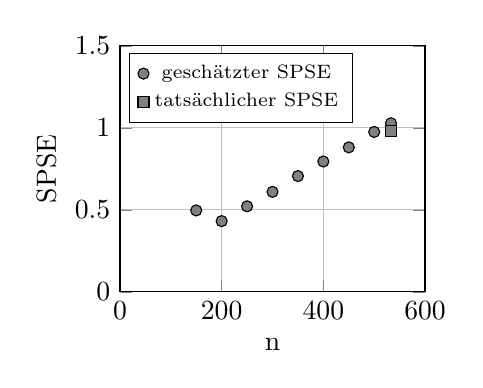
\begin{tikzpicture}
        \begin{axis}[ 
            ylabel = SPSE,
            xlabel = n,
            xmin=0, xmax=600,
            ymin=0, ymax=1.5,
            legend pos = north west,
            scaled ticks = false,
            width = .45\textwidth,
            ymajorgrids,
            xmajorgrids,
            %height = 8cm,
            cycle list name=black white
        ]
            \addplot +[only marks]
            coordinates {
                (150,0.4964226)
                (200,0.4312206)
                (250,0.5213190)
                (300,0.6097658)
                (350,0.7058959)
                (400,0.7947748)
                (450,0.8807918)
                (500,0.9750933)
                (533,1.0280917)
            };
            \addlegendentry{{\scriptsize geschätzter SPSE}}
            
            \addplot +[only marks]
            coordinates {
                (533,0.9813258)
            };
            \addlegendentry{{\scriptsize tatsächlicher SPSE}}
        \end{axis}
    \end{tikzpicture}
    \captionof{figure}{geschätzer sowie tatsächlicher SPSE in Abhängigkeit der Stichprobengröße}
    \label{fig:spse}
\end{figure}